%%%%%%%%%%%%%%%%%%%% book.tex %%%%%%%%%%%%%%%%%%%%%%%%%%%%%
%
% sample root file for the chapters of your "monograph"
%
% Use this file as a template for your own input.
%
%%%%%%%%%%%%%%%% Springer-Verlag %%%%%%%%%%%%%%%%%%%%%%%%%%


% RECOMMENDED %%%%%%%%%%%%%%%%%%%%%%%%%%%%%%%%%%%%%%%%%%%%%%%%%%%
\documentclass[envcountsame,envcountchap]{svmono}
\usepackage{ctex}  %中文

% choose options for [] as required from the list
% in the Reference Guide, Sect. 2.2
\usepackage{epstopdf}
\usepackage{makeidx}         % allows index generation
\usepackage{graphicx}        % standard LaTeX graphics tool
                             % when including figure files
\usepackage{multicol}        % used for the two-column index
\usepackage[bottom]{footmisc}% places footnotes at page bottom
% etc.
% see the list of further useful packages
% in the Reference Guide, Sects. 2.3, 3.1-3.3

\makeindex             % used for the subject index
                       % please use the style svind.ist with
                       % your makeindex program

                     
%%%%%%%%%%%%%%%%%%%%%%%%%%%%%%%%%%%%%%%%%%%%%%%%%%%%%%%%%%%%%%%%%%%%%
\usepackage{geometry}
\geometry{left=2.5cm,right=2.5cm,top=2.5cm,bottom=2.5cm}
\usepackage{amsmath}

\usepackage{hyperref}
\usepackage[all]{hypcap}
\usepackage{enumerate}

\begin{document}

% \author{Author(s)}
% \title{Insert your Booktitle, Subtitle, Edition\\
% {\small SPIN Springer's internal project number, if known}}
% \subtitle{-- Monograph --}
% \maketitle

% \frontmatter%%%%%%%%%%%%%%%%%%%%%%%%%%%%%%%%%%%%%%%%%%%%%%%%%%%%%%

% \include{dedic}
% \include{pref}
% \tableofcontents


\mainmatter%%%%%%%%%%%%%%%%%%%%%%%%%%%%%%%%%%%%%%%%%%%%%%%%%%%%%%%
\include{part}
%%%%%%%%%%%%%%%%%%%%% chapter.tex %%%%%%%%%%%%%%%%%%%%%%%%%%%%%%%%%
%
% Calibration chapter
%
%
%%%%%%%%%%%%%%%%%%%%%%%% Springer-Verlag %%%%%%%%%%%%%%%%%%%%%%%%%%

\chapter{传感器标定}
\label{intro} % Always give a unique label
\label{sec:1}

LiDAR和相机联合标定是确定车载LiDAR和相机间的刚体变换关系,对齐3D点云和2D像素,为多传感器数据融合提供基础。
标定的关键是寻找在LiDAR和相机视野内的匹配模式。
考虑到标定的可操作性和精确度,以及后续标定误差的矫正,
我们首先采用传统的基于平面靶的标定方法,快速获取6DOF外参;然后基于边缘匹配在线更新外参,获取更高精度的
外参。


\begin{figure*}
\begin{center}
    \includegraphics[width=14cm]{fig/coord.pdf} \\
    \caption{(1)LiDAR 和相机坐标系 (2)像平面坐标系 (3)成像模型 (4)图像坐标系与相机坐标系}
    \label{fig: coordinate}
\end{center}
\end{figure*}

\section{LiADR-Camera联合粗标定}

为描述车载传感器的相对位置关系,建立如\figurename\ref{fig: coordinate} (1)坐标系
(所有坐标系均为右手系),并引入中间坐标系(世界坐标系)来建立相机内标定和LiDAR-Camera系统外标定
间的联系。其中Velodyne 64HDL LiDAR 坐标系定义$X_{l}$轴指向车身正前方,$Z_{l}$轴垂直向上;
定义相机坐标系$Z_{c}$轴指向车身正前方,$Y_{c}$轴垂直向下。


\subsection{从空间点到像平面坐标系}
如\figurename\ref{fig: coordinate} (2)所示,图像坐标系(像素坐标系),以图像左上角的顶点$O_{0}$
为原点, $(u,v)$为像素坐标。像平面坐标系(物理坐标系),以摄像机光轴与图像平面的交点$O_{1}$为原点,
$(x,y)$为像平面坐标。相机理想的成像过程如 \figurename\ref{fig: coordinate} (3)(4)所示,
世界坐标系下点P$(X_{w},Y_{w},Z_{w})$经坐标变换到相机坐标系下$P^{'}(X_{c},Y_{c},Z_{c})$后,
透视变换投影到图像平面,变换过程模型如下:
\begin{equation}
\begin{aligned}
\begin{bmatrix} u \\v\\1 \end{bmatrix}=
\begin{bmatrix} f_{x} & 0 & u_{0} & 0 \\0 & f_{y} & v_{0} & 0\\0 & 0 & 1 & 0 \end{bmatrix}         
\begin{bmatrix} \vec{R_{c}} & \vec{t_{c}}\\ \vec{0}^{T} & 1 \end{bmatrix}
\begin{bmatrix} X_w \\Y_w\\Z_w \end{bmatrix}
\end{aligned}
\end{equation}
式中,$f_{x}$和$f_{y}$表示沿图像坐标系的x轴和y轴方向上单位长度的像素值,与像平面主点$u_{0}$和$v_{0}$一起构成
相机内参;$\vec{R_{c}}$ 和$\vec{t_{c}}$分别为世界坐标系到相机坐标系的旋转矩阵和平移矩阵。

采集标定板数据(\figurename\ref{fig: calib}),利用张正友标定法标定相机内参时,可以得到标定板在相机坐标系下的位姿,
因此定义世界坐标系$Z_{w}$轴与相机光轴重合(垂直于标定板),$O-X_{w}Y_{w}$平面与标定板重合,对于n帧标定
数据,就可以得到n对$\vec{R_{ci}}$和$\vec{t_{ci}}$矩阵;将正交旋转矩阵用“角-轴”的方式表示就能得到
旋转角$\theta_{c,i}$,并由平移量得到标定板相对于相机原点的距离$\alpha_{c,i}$。

\begin{figure*}[htbp]
	\centering
    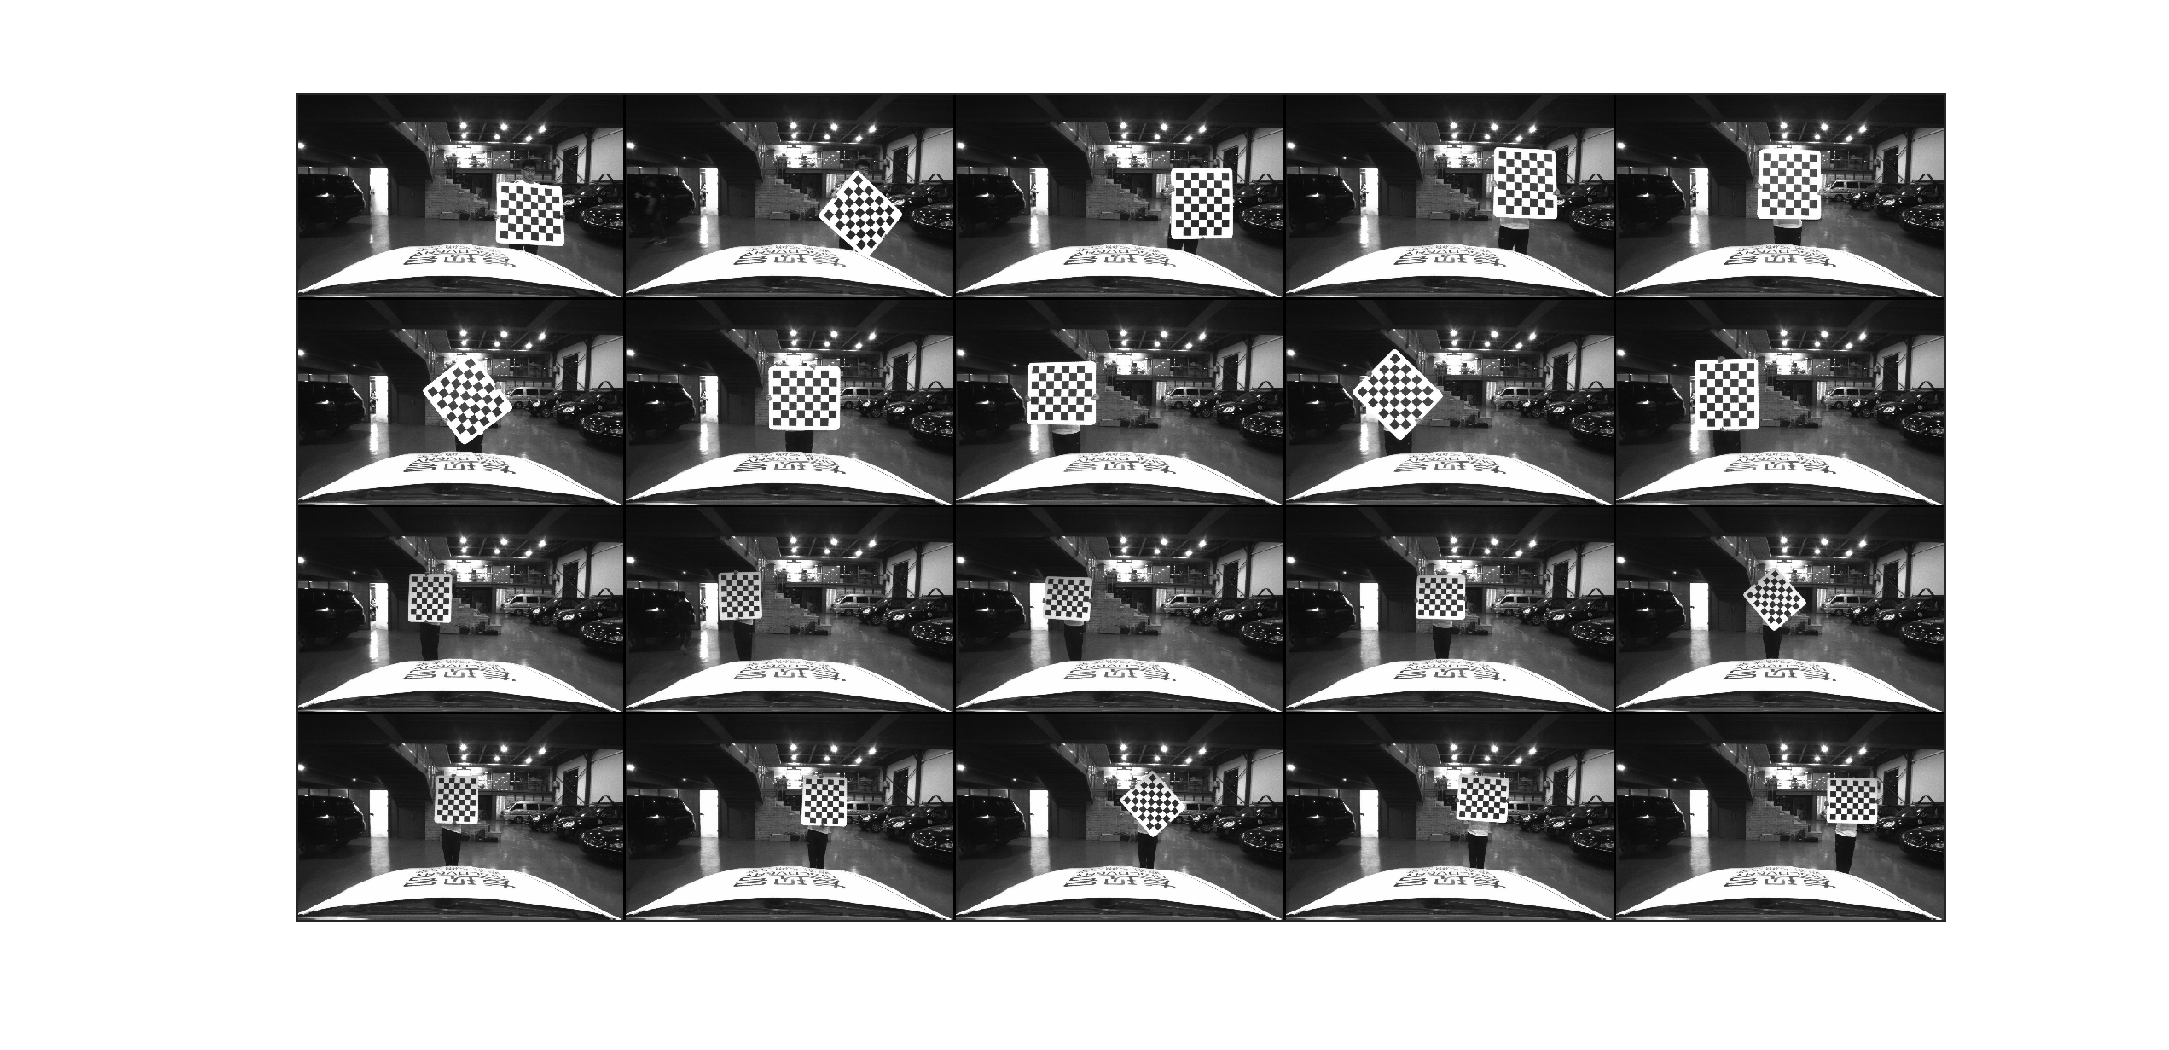
\includegraphics[width=16cm]{fig/data1.eps} \\
	\caption{标定板数据}\label{fig: calib}
\end{figure*}

\subsection{从LiDAR坐标系到相机坐标系}
已知标定板(世界坐标系)在相机坐标系下的位姿,要求解LiDAR坐标系和相机坐标系间的刚体变换关系,首先需得到LiDAR坐标系和
标定板间的刚体变换关系,因此,我们手动提取标定板的点云数据,并用最小二乘法进行拟合,得到该平面在LiDAR坐标系下位姿估计值
的“角-轴”值,即$\theta_{l,i}$和$\alpha_{l,i}$。然后,以LiDAR坐标系和相机坐标系下各标定平面到相机坐标系原点的
距离差的最小值为目标函数,优化该目标函数得到最优平移量,最后以LiDAR坐标系和相机坐标系下各标定平面到相机坐标系原点的
法向量夹角的最小值为目标函数,优化该目标函数得到最优旋转量。

相机坐标系原点平移t(LiDAR与相机间的距离)后,相机距标定平面的距离为$\alpha_{c,i}-\theta_{c,i}^{T}t$,
所以与平移量有关的目标函数如下:
\begin{equation}\label{eq1}
\begin{aligned}
& \min \limits_{t} \sum_{i=1}^{n}(\alpha_{l,i}-(\alpha_{c,i}-\theta_{c,i}^{T}t))^{2} \\
\Longrightarrow & t_{1}=\arg \min \limits_{t} || (\theta_{c}^{T}t-(\alpha_{l}-\alpha_{c}))||^{2}_{F} \\
\end{aligned}
\end{equation}
解 \eqref{eq1}, 即可得到平移量
$t_{1}=(\theta_{c}\theta_{c}^{T})^{-1}\theta_{c}(\alpha_{c}-\alpha_{l})$。

法向量夹角的最小值即夹角余弦的最大值,用正交旋转矩阵表示,则与旋转量有关的目标函数如下:
\begin{equation}\label{eq2}
\begin{aligned}
R_{1}=\arg \max \limits_{R} \sum_{i=1}^{n} \theta_{c,i}^{T} (R \theta_{l,i})
\end{aligned}
\end{equation}
其中,R是正交旋转矩阵,满足$R^{T}R=\vec{I}_{3}$,$det(R)=1$,对公式 \eqref{eq2}变形,将该问题转换成
典型的正交普鲁克问题(Orthogonal Procrustes Problem),如式下所示。
\begin{equation}\label{eq3}
\begin{aligned}
R_{1}=\max \limits_{R} trace(\theta_{c}^{T}R\theta_{l})
=\max \limits_{R} trace(R\theta_{l}\theta_{c}^{T})
\end{aligned}
\end{equation}
用奇异值分解(Singular Value Decomposition,SVD)的方法解\eqref{eq3},即可以得到旋转矩阵的解:
\begin{equation}
\begin{aligned}
R_{1}= VU^{T},  st.\theta_{l}\theta_{c}^{T}=USV^{T}
\end{aligned}
\end{equation}

以上的求解过程,我们仅使用点云数据估计了标定板平面参数值,为了更有效地利用点云数据并提高算法的鲁棒性,
我们使用点云平面拟合得到的内点进一步对上述过程中得到的LiDAR-Camera系统外参进行优化。

用$x_{l,i}$表示第i帧点云中拟合的标定板平面的内点,
即$x_{l,i}=[x_{l,i}^{(1)}, x_{l,i}^{(2)},...,x_{l,i}^{(m)}]$,$x_{l,i} \in R^{3x1}$,$m=m(i)$是
第i帧点云中拟合平面得到的内点的个数,则建立的统一旋转和平移量的目标函数如\eqref{eq4}所示,以上述$R_{1}$和$t_{1}$
为初值,优化该问题,得到粗标定过程的最终外参矩阵。
\begin{equation}\label{eq4}
\begin{aligned}
\arg \max \limits_{R,t} \sum_{i=1}^{n}\frac{1}{m(i)} 
\sum_{j=1}^{m(i)} (\theta_{c,i}^{T} (R x_{l,i}^{(j)}+t)-\alpha_{c,i})^{2}
\end{aligned}
\end{equation}

%%%%%%%%%%%%%%%%%%%%%%%%%%%%%%%%%%%%%%%%%%%%%%%%%%%%%%%%%%%%%%%%%%%%%%%%%%%%%%%%%%%%%%%%%
\section{LiADR-Camera联合细标定}
\label{sec:2}
将相机内参标定和LiDAR-Camera联合标定过程统一, 均使用棋盘格为靶标,方便采集实验数据,并降低了实验要求,简化了整个
标定流程。这种基于黑白棋盘格的离线标定方法虽然简单易实现,但是仍存在一些问题:
\begin{enumerate}[\indent (1)]
\item 标定精度难以保证;标定受光照和人为因素影响大,很多情况下的标定结果都不能满足后续点云和图像高精度融合的需要。
\item 标定误差无法更新和校正;这种基于特定靶标的离线标定方法,一旦标定结果发生偏移,都需要重新实验,过程繁琐,
无法满足无人驾驶系统在线感知算法的需求。
\end{enumerate}

综合考虑以上问题,我们用真实道路场景中的目标(人,树,路标,车等)作为LiDAR-Camera系统外标定的匹配模式,基于点云和图像
目标边缘对齐的融合结果,在线优化和更新该传感器系统外参。


\subsection{数据处理}
% 为保证所选点云和图像对边缘特征明显易于提取,需要人为选择数据采集场景或者人为对时间同步后的数据进行筛选。
3D点云和2D图像数据模态存在巨大差异,在进行边缘提取前,需先对点云减采样,取与相机视野重合扇区内的点云;并对点云进行
简单滤波,除去地面点(基于高度的滤波或者RANSAC)和非目标点(基于距离滤波或者检测算法)。然后,剪裁RGB图像,除去LiDAR
激光器扫描到的最高高度以外的图像区域,并根据图像剪裁的尺寸更新相机内参。最后处理得到如
\figurename\ref{fig: IDT-FIL}所示的图像和点云边缘。

\begin{figure*}[htbp]
	\centering
    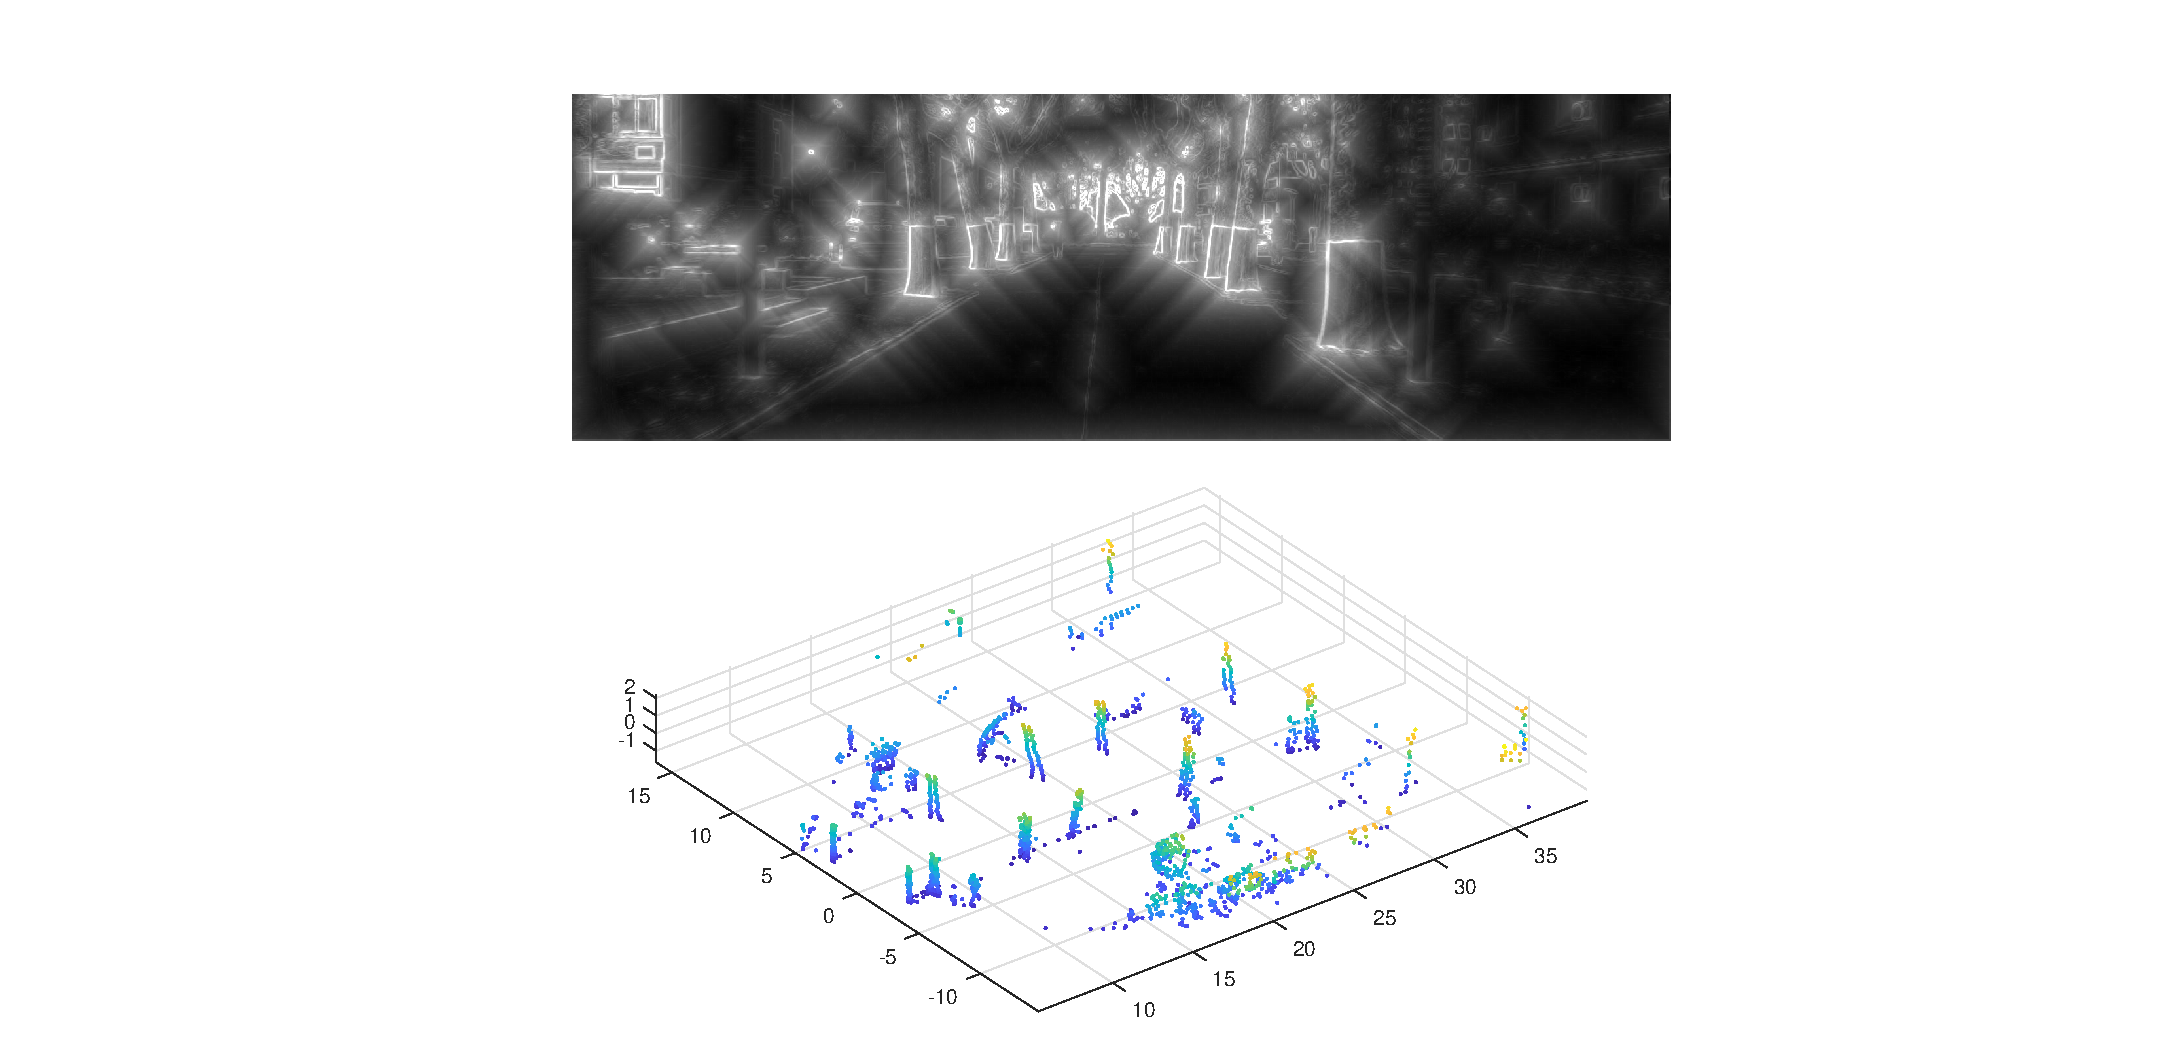
\includegraphics[width=18cm]{fig/IDT.eps} \\
	\caption{图像和点云边缘提取结果}\label{fig: IDT-FIL}
\end{figure*}

\subsubsection{点云边缘提取}
3D点云数据离散而稀疏,边缘不连续性明显,因此利用点云数据获取的边缘存在误差(与点云的分辨率有关)。
我们单独分析每帧点云中的每个激光器的返回数据,对于场景中的目标,由于视差和遮挡,则具有固定垂直扫射角的激光器的
返回数据中,与左右邻域点相比,越远的点越不可能是目标边缘点。基于该事实,建立式 \eqref{eq5}的点云边缘滤波指标。
\begin{equation}\label{eq5}
\begin{aligned}
X_i=\max(P_{i-1}^{r}-P_{i}^{r}, P_{i}^{r}-P_{i+1}^{r}, 0)^\gamma
\end{aligned}
\end{equation}
其中,$P_{i}^{r}$是返回的第i个点的深度值,$\gamma \in(0, 1)$是为提高近处点云权重而设置的参数,一般取经验值0.5。

对于Velodyne 64HDL LiDRA点云数据,我们以$X_i\ge 0.3m$为基准滤波提取点云数据中目标的边缘。


\subsubsection{图像边缘提取}
与点云边缘检测算法相比,图像边缘检测算法成熟,检测精度高,但仍然存在一些影响边缘匹配的问题,诸如由光照和阴影导致的
假边缘、离散孤立边,这些边难以滤波去除,因此除了人为选择标定场景(无强光和阴影的阴天或者傍晚等)外,我们对得到的边缘
图进行距离逆变换(inverse distance transform, IDT),提高真实边缘的比重并弥补点云边缘不连续性导致的边缘误差。
我们首先使用Sobel算子提取图像边缘,得到边缘图E,然后对E做IDT变换,变换过程如下:
\begin{equation}
\begin{aligned}
D_{i,j}=\alpha \cdot E_{i,j}+(1-\alpha)\cdot \max \limits_{x,y} E_{x,y}
\cdot \mu^{\max(|x-i|,|y-j|)} 
\end{aligned}
\end{equation}
其中,i, j, x, y为图像边缘E的像素索引,$\alpha$和$\mu$分别取经验值0.333和0.98。

\subsection{基于边缘匹配更新外参}
将粗标定过程中得到的旋转外参矩阵转换为欧拉角表示可以得到LiDAR-Camera系统的6DOF外参,
$C=(t_{x},t_{y},t_{z},\theta_{x},\theta_{y},\theta_{z})$,以此为初值,将点云投影到图像平面
可以建立与6DOF外参有关的目标函数,如下:
\begin{equation}\label{eq6}
\begin{aligned}
F_T=\sum_{f=1}^{n} \sum_{p=1}^{X^{f}} X_{p}^{f}\cdot D_{i,j}^{f}
\end{aligned}
\end{equation}
其中,n是选择用于实验的点云图像对的数量,$X^{f}$表示预处理后第f帧点云数据中点的个数,$(i,j)$表示第p个点投影到图像
平面的位置索引。

我们使用邻域搜索算法求解问题\eqref{eq6},得到更精确的外参。

%%%%%%%%%%%%%%%%%%%%%%%%%%%%%%%%%%%%%%%%%%%%%%%%%%%%%%%%%%%%%%%%%%%%%%%%%%%%%%%%%%%%%%
\section{标定流程}
\label{sec:3}

\subsection{数据采集与预处理}
\subsubsection{数据采集}

标定操作在MATLAB环境下进行,在Calibration文件夹下,包含CoarseCalibration、FineSearch、fToolBox、LCCT1、TOOLBOX$\_$calib五个文件夹。
CoarseCalibration文件夹下主要包含了img$\_$veloPreprocess.m和show.m两个文件,img$\_$veloPreprcoess根据筛选出的的图片来产生图片和点云对,show根据得到的标定矩阵来显示标定的结果。
FineSearch文件夹下主要包含了dataPreprocess.m和Search.m两个文件,dataPreprocess用来生成细标定搜索使用的数据,Search用来根据粗标定得到的结果和已有数据进一步优化标定矩阵,使之更为准确。
fToolBox文件夹主要包含了timeAlign.m,timeAlign用来对采集到的数据进行时间对齐并按时间顺序标号。
LCCT1文件夹为外参粗标定使用的工具箱文件夹。


TOOLBOX$\_$calib文件夹为相机内参标定使用的工具箱的文件夹。

% 在同样距离等条件下,激光对于白色材料反射强度最高,检测到的数据准确率最高。要求采集的标定板数据标定板平坦且边缘整齐。
% 我们采用的是7*8个边长为100mm的格子的标定板。

% 标定时保证相机与雷达前方区域平坦且光照条件柔和,无强光照射标定板。
% 将标定板朝向相机,以间距约0.5,1.5,2.5m围绕相机前方各个位置采集标定数据。

% 在VisualStudio下分别使用图像采集程序
% (img.cpp)与雷达数据采集程序(hdl.cpp)两个程序采集数据。

\subsubsection{时间同步}
采集数据后,使用MATLAB对数据进行预处理。首先进行时间同步:

\begin{enumerate}[$\star$]%项目符号开始
\item 使用文件: fToolBox$\verb|\|$timeAlign.m;
\item 部分代码片段如\figurename\ref{fig: timeAlign}所示;
\item 改其中的路径Path为存储标定数据的根文件夹;
\item 该程序会自动在根文件下创建dataSet文件夹,其中dataSet文件夹又包含img、velo、target、img$\_$select
四个子文件夹,分别用来存储时间对齐后的图像、时间对齐后的点云、筛选出用来标定的图片和点云对、筛选出的图片;
\item 点击“Run”运行,即可完成时间对齐,图像和点云分别以img$\_$xxxxxx.jpg和velo$\_$xxxxxx,
(xxxxxx为时间戳顺序的编号)存储在img和velo文件夹下。
\end{enumerate}

\begin{figure*}[htbp]
	\centering
    \includegraphics[width=12cm]{pic/TAL.png} \\
	\caption{时间同步代码片段}\label{fig: timeAlign}
\end{figure*}

\subsubsection{选取图片}
\begin{enumerate}[$\star$]%项目符号开始
\item 在img文件夹下,人工选择各个位置下的光照良好标定板无亮斑且边缘整齐的图片约40张放入img$\_$select文件夹内;
\item 使用MATLAB相机标定工具箱Camera Calibrator,图标与界面如\figurename\ref{fig: caca}所示。
\end{enumerate}

\begin{figure*}[htbp]
	\centering
    \includegraphics[width=8.5cm]{pic/2.png} \\
	\caption{Camera Calibrator图标与界面}\label{fig: caca}
\end{figure*}

具体操作流程如下:
% \begin{enumerate}[\indent $1)$]
% \item Add Images添加img$\_$select文件夹下的图片,点击“打开”;
% \item 弹出窗口如图3所示,Size of checkerbored square为标定板格子的边长,设定为100mm,点击“确定”;
% \item 点击Calibrate进行标定运算;
% \item 选择右侧Reprojection Errors中值较高的图片,即为我们可以筛掉的图片。
% 每次选择Reprojection Errors最高的一张图片,在img$\_$select文件夹中将其删除,并在界面中右键选择对应照片,
% 点击“Remove and Recalibrate”重新进行运算,如图4所示;
% \item 最后保留28-35张图片;
% \item 点击“Export Camera Parameters”保存工具箱计算得到的相机内参,为后续标定作参考;
% \end{enumerate}
\begin{enumerate}[\indent $1)$]
\item Add Images添加img$\_$select文件夹下的图片,点击“打开”;
\item 弹出窗口如\figurename\ref{fig: pic3}所示,Size of checkerbored square为标定板格子的边长,设定为100mm,点击“确定”;
\end{enumerate}

\begin{figure*}[htbp]
	\centering
    \includegraphics[width=8.5cm]{pic/3.png} \\
	\caption{设定标定板格子边长}\label{fig: pic3}
\end{figure*}

\begin{enumerate}[\indent $3)$]
\item 点击Calibrate进行标定运算;
\end{enumerate}

\begin{enumerate}[\indent $4)$]
\item 选择右侧Reprojection Errors中值较高的图片,即为我们可以筛掉的图片。
每次选择Reprojection Errors最高的一张图片,在img$\_$select文件夹中将其删除,并在界面中右键选择对应照片,
点击“Remove and Recalibrate”重新进行运算,如\figurename\ref{fig: pic4}所示;
\end{enumerate}

\begin{figure*}[htbp]
	\centering
    \includegraphics[width=12cm]{pic/4.png} \\
	\caption{删除图片并重新运算}\label{fig: pic4}
\end{figure*}

\begin{enumerate}[\indent $5)$]
\item 最后保留28-35张图片;
\end{enumerate}

\begin{enumerate}[\indent $5)$]
\item 点击“Export Camera Parameters”保存工具箱计算得到的相机内参,为后续标定作参考。
\end{enumerate}

图片筛选完成后,进行如下操作来生成最终标定使用的图片点云对:
\begin{enumerate}[$\star$]
\item 使用文件: CoarseCalibration$\verb|\|$img$\_$veloPreprocess.m,部分代码片段如\figurename\ref{fig: pic5}所示;
\item 修改其中的路径Path为标定数据文件夹下的dataSet文件夹;
\item 点击“Run”运行,即可找到选出的图片的对应激光点云,并保存在target文件夹里,
名称为laser$\_$targetX.xyz和img$\_$targetX.jpg。
\end{enumerate}

\begin{figure*}[htbp]
	\centering
    \includegraphics[width=8cm]{pic/5.png} \\
	\caption{img$\_$veloPreprocess部分代码片段}\label{fig: pic5}
\end{figure*}


\subsection{相机内参标定}
使用标定工具箱Matlab Calibration Toolbox:
\begin{enumerate}[$\star$]
\item 右键选择TOOLBOX$\_$calib文件夹,添加到路径$\rightarrow$选定的文件夹和子文件夹;
\item 将MATLAB当前文件夹设为target文件夹;
\item 命令行输入calib$\_$gui,出现界面如\figurename\ref{fig: pic6}所示,选择“Standard”;
\end{enumerate}

\begin{figure*}[htbp]
	\centering
    \includegraphics[width=8cm]{pic/6.png} \\
	\caption{初始界面}\label{fig: pic6}
\end{figure*}

\begin{enumerate}[$\star$]
\item 出现界面如\figurename\ref{fig: pic7}所示,选择“Image Names”;
\end{enumerate}

\begin{figure*}[htbp]
    \centering
    \includegraphics[width=10cm]{pic/7.png} \\
    \caption{工具箱界面}\label{fig: pic7}
\end{figure*}

\begin{enumerate}[$\star$]
\item 命令行出现“Basename camera calibration images (without number nor suffix):”,
此时需要输入图像基础名称,所以在命令行输入“img$\_$target”,回车;
\item 命令行出现“Image format: ([]='r'='ras', 'b'='bmp', 't'='tif', 'p'='pgm', 'j'='jpg', 'm'='ppm')”,
此时需要选择图像格式,所以输入“j”,回车;
\item 图片加载完成后,选择“Extract Grid Corners”,命令行出现“Number(s) of image(s) to process
 ([] = all images) =”,回车默认选择全部图片;
\item 命令行出现“wintx ([] = 15) =”和“winty ([] = 15) =”,即为选择窗口大小,两次回车即可;
\item 命令行出现“Do you want to use the automatic square counting mechanism 
(0=[]=default)or do you always want to enter the number of squares manually (1,other)?”,回车即可;
\item 弹出窗口中,接下来需要选择标定板的四个角点,选定其中一角作为原点,每次按照该原点按顺时针围一个框,
如\figurename\ref{fig: pic8}(1)所示,选好后回车确认,命令行出现“Size dX of each square along the X direction 
([]=100mm) =  Size dY of each square along the Y direction ([]=100mm) =”,回车确认,
此时出现角点检测后的结果,如\figurename\ref{fig: pic8}(2)所示
\end{enumerate}

\begin{figure*}[htbp]
    \centering
    \includegraphics[width=14cm]{pic/8.pdf} \\
    \caption{(1)选择标定板角点 (2)角点检测结果}\label{fig: pic8}
\end{figure*}

\begin{enumerate}[$\star$]
\item 命令行出现“Need of an initial guess for distortion? ([]=no, other=yes)”,
再次回车出现下一张图,重复上述操作直到所有图片检测完毕;
\item 选择“Calibration”进行相机内参标定运算;
\item 选择“Save”,保存结果,会在target文件夹下生成名称为Calib$\_$Result.mat的文件。
\end{enumerate}

\subsection{LiDRA-Camera联合粗标定}
使用LCCT工具箱标定LiDRA-Camera系统初始外参:

\begin{enumerate}[$\star$]
\item 右键选择LCCT1下的src文件夹,添加到路径$\rightarrow$选定的文件夹和子文件夹;
\item 将MATLAB当前文件夹设为target文件夹;
\item 命令行输入lasercamcalib,出现界面如\figurename\ref{fig: pic9}所示;
\item 选择“Select a camera calib file”,选择Calib$\_$Result.mat;
\item 选择“Search scan files”,命令行出现“Enter base name of scans (without numbers or suffix):”,
即选择点云文件基础名称,输入laser$\_$target,回车;
\item 命令行出现“Enter suffix of scan files ([] = "xyz"):”,即选择点云文件扩展名,直接回车即可;
\item 选择“List active”;
\item 选择“Select planes”,命令行出现“Enter indices of range images to preview ([]=all active):”,
直接回车即可;
\item 命令行出现“use range image (r) or 3D point cloud (p) to select checkboard plane?
 (default:p):”,此时需要选择选定标定板的方法,我们选择rang image的方式,故输入r,回车;
\end{enumerate}

\begin{figure*}[htbp]
    \centering
    \includegraphics[width=6cm]{pic/9.png} \\
    \caption{LCCT工具箱界面}\label{fig: pic9}
\end{figure*}

\begin{enumerate}[$\star$]
\item 出现图片窗口如\figurename\ref{fig: pic10}所示,选择Select plane,左键选择标定板角点,
ESC可以取消之前的选定,选好后右键确认;
\end{enumerate}

\begin{figure*}[htbp]
    \centering
    \includegraphics[width=9cm]{pic/10.png} \\
    \caption{选择标定板平面区域}\label{fig: pic10}
\end{figure*}

\begin{enumerate}[$\star$]
\item 选择“Next”,然后重复操作,直至处理完所有图片;
\item 选择“Save$\&$Quit”;
\item 在工具箱界面选择“Calibrate”进行标定运算;
\item 选择“Save”,输入要保存的名字,回车即可保存。
\end{enumerate}

\subsection{LiDRA-Camera联合细标定}
执行搜索算法前,先处理用于搜索的数据:
\begin{enumerate}[$\star$]
\item 预选选取5-15对时间同步后边缘明显的点云-图像数据,保存在FineSearch$\verb|\|$Data$\verb|\|$ORGData目录中;
\item 运行FineSearch目录下数据处理文件dataPreprocess.m,调用IDT.m函数处理图像,
调用PC$\_$filter.m函数处理点云,将得到的图像边缘和点云边缘保存于结构体数据Data.mat中,
存于FineSearch$\verb|\|$Data目录下;
\item 调用自定义工具箱fToolBox中Rt2C.m将粗标定过程中得到的外参矩阵用6DOF外参C表示;
\end{enumerate}

得到图像和点云边云后,使用搜索算法精确标定传感器系统外参:

\begin{enumerate}[$\star$]
\item 初始化FineSearch目录下Search.m函数中的内参K$\_$int和外参C;
\item 更新搜索步长delta$\_$t和delta$\_$R;
\item 执行Search.m文件;
\item 搜索的关键代码片段如\figurename\ref{fig: pic11}所示。
\end{enumerate}

\begin{figure*}[htbp]
    \centering
    \includegraphics[width=13cm]{pic/11.png} \\
    \caption{Search.m代码片段}\label{fig: pic11}
\end{figure*}

%%%%%%%%%%%%%%%%%%%%%%%%%%%%%%%%%%%%%%%%%%%%%%%%%%%%%%%%%%%%%%%%%%%%%%%%%%%%%%%%%%%%%%%%%%%
\section{标定注意事项}

\begin{enumerate}[\indent $1)$]
\item 制作棋盘格靶标时应特别注意,黑色方格与白色方格尺寸需要相同,而且所有方格的尺寸必须严格一致。
靶标的方格数量不宜太小,行数和列数以大于7为宜。方格的尺寸不宜太大或太小,采集的整幅靶标图像中方格的边长尺寸不小于
20像素。
\item 采集靶标图像时应特别注意,需要在不同的角度不同的位置采集靶标的多幅图像。
采集到的图像必须清晰,靶标图像尺寸以占整幅图像尺寸的1/3-3/4为宜。靶标
图像最好在整幅图像的不同位置都有分布,不宜过于集中于同一区域。靶标放置位
置与摄像机之间的距离最好为视觉系统的主要工作距离。靶标相对于摄像机的角度
应有较大范围的变化,应包含绕三个轴较大角度的旋转,最好不小于30度。采集
的靶标图像数量不应太少,建议以20-35幅靶标图像为宜。
\item 内参标定,提取角点时,在图形窗口利用鼠标点击设定棋盘格靶标的选定区域。点击的第一个
角点作为靶标坐标系的原点,顺序点击 4 个角点形成四边形。相邻两次点击的角点应在同一条网格线上,
使得所形成的四边形的边应与棋盘格靶标的网格线基本平行。为提高点击的角点的精度,
建议将显示靶标图像的图像窗口放大到最大,利用
鼠标的十字标线尽可能准确的点击4个角点。
\item 外参标定,提取角点时,在图形窗口利用鼠标点击的第一个角点作为靶标坐标系的原点,得到
的外参数是靶标坐标系在摄像机坐标系中的位姿。
\item 采集细标定数据时,避免强光和阴影,建议傍晚和阴天采集数据。
\end{enumerate}

%%%%%%%%%%%%%%%%%%%%%% chapter.tex %%%%%%%%%%%%%%%%%%%%%%%%%%%%%%%%%
%
% Calibration chapter
%
%
%%%%%%%%%%%%%%%%%%%%%%%% Springer-Verlag %%%%%%%%%%%%%%%%%%%%%%%%%%

\chapter{传感器标定}
\label{intro} % Always give a unique label
\label{sec:1}

LiDAR和相机联合标定是确定车载LiDAR和相机间的刚体变换关系,对齐3D点云和2D像素,为多传感器数据融合提供基础。
标定的关键是寻找在LiDAR和相机视野内的匹配模式。
考虑到标定的可操作性和精确度,以及后续标定误差的矫正,
我们首先采用传统的基于平面靶的标定方法,快速获取6DOF外参;然后基于边缘匹配在线更新外参,获取更高精度的
外参。


\begin{figure*}
\begin{center}
    \includegraphics[width=14cm]{fig/coord.pdf} \\
    \caption{(1)LiDAR 和相机坐标系 (2)像平面坐标系 (3)成像模型 (4)图像坐标系与相机坐标系}
    \label{fig: coordinate}
\end{center}
\end{figure*}

\section{LiADR-Camera联合粗标定}

为描述车载传感器的相对位置关系,建立如\figurename\ref{fig: coordinate} (1)坐标系
(所有坐标系均为右手系),并引入中间坐标系(世界坐标系)来建立相机内标定和LiDAR-Camera系统外标定
间的联系。其中Velodyne 64HDL LiDAR 坐标系定义$X_{l}$轴指向车身正前方,$Z_{l}$轴垂直向上;
定义相机坐标系$Z_{c}$轴指向车身正前方,$Y_{c}$轴垂直向下。


\subsection{从空间点到像平面坐标系}
如\figurename\ref{fig: coordinate} (2)所示,图像坐标系(像素坐标系),以图像左上角的顶点$O_{0}$
为原点, $(u,v)$为像素坐标。像平面坐标系(物理坐标系),以摄像机光轴与图像平面的交点$O_{1}$为原点,
$(x,y)$为像平面坐标。相机理想的成像过程如 \figurename\ref{fig: coordinate} (3)(4)所示,
世界坐标系下点P$(X_{w},Y_{w},Z_{w})$经坐标变换到相机坐标系下$P^{'}(X_{c},Y_{c},Z_{c})$后,
透视变换投影到图像平面,变换过程模型如下:
\begin{equation}
\begin{aligned}
\begin{bmatrix} u \\v\\1 \end{bmatrix}=
\begin{bmatrix} f_{x} & 0 & u_{0} & 0 \\0 & f_{y} & v_{0} & 0\\0 & 0 & 1 & 0 \end{bmatrix}         
\begin{bmatrix} \vec{R_{c}} & \vec{t_{c}}\\ \vec{0}^{T} & 1 \end{bmatrix}
\begin{bmatrix} X_w \\Y_w\\Z_w \end{bmatrix}
\end{aligned}
\end{equation}
式中,$f_{x}$和$f_{y}$表示沿图像坐标系的x轴和y轴方向上单位长度的像素值,与像平面主点$u_{0}$和$v_{0}$一起构成
相机内参;$\vec{R_{c}}$ 和$\vec{t_{c}}$分别为世界坐标系到相机坐标系的旋转矩阵和平移矩阵。

采集标定板数据(\figurename\ref{fig: calib}),利用张正友标定法标定相机内参时,可以得到标定板在相机坐标系下的位姿,
因此定义世界坐标系$Z_{w}$轴与相机光轴重合(垂直于标定板),$O-X_{w}Y_{w}$平面与标定板重合,对于n帧标定
数据,就可以得到n对$\vec{R_{ci}}$和$\vec{t_{ci}}$矩阵;将正交旋转矩阵用“角-轴”的方式表示就能得到
旋转角$\theta_{c,i}$,并由平移量得到标定板相对于相机原点的距离$\alpha_{c,i}$。

\begin{figure*}[htbp]
	\centering
    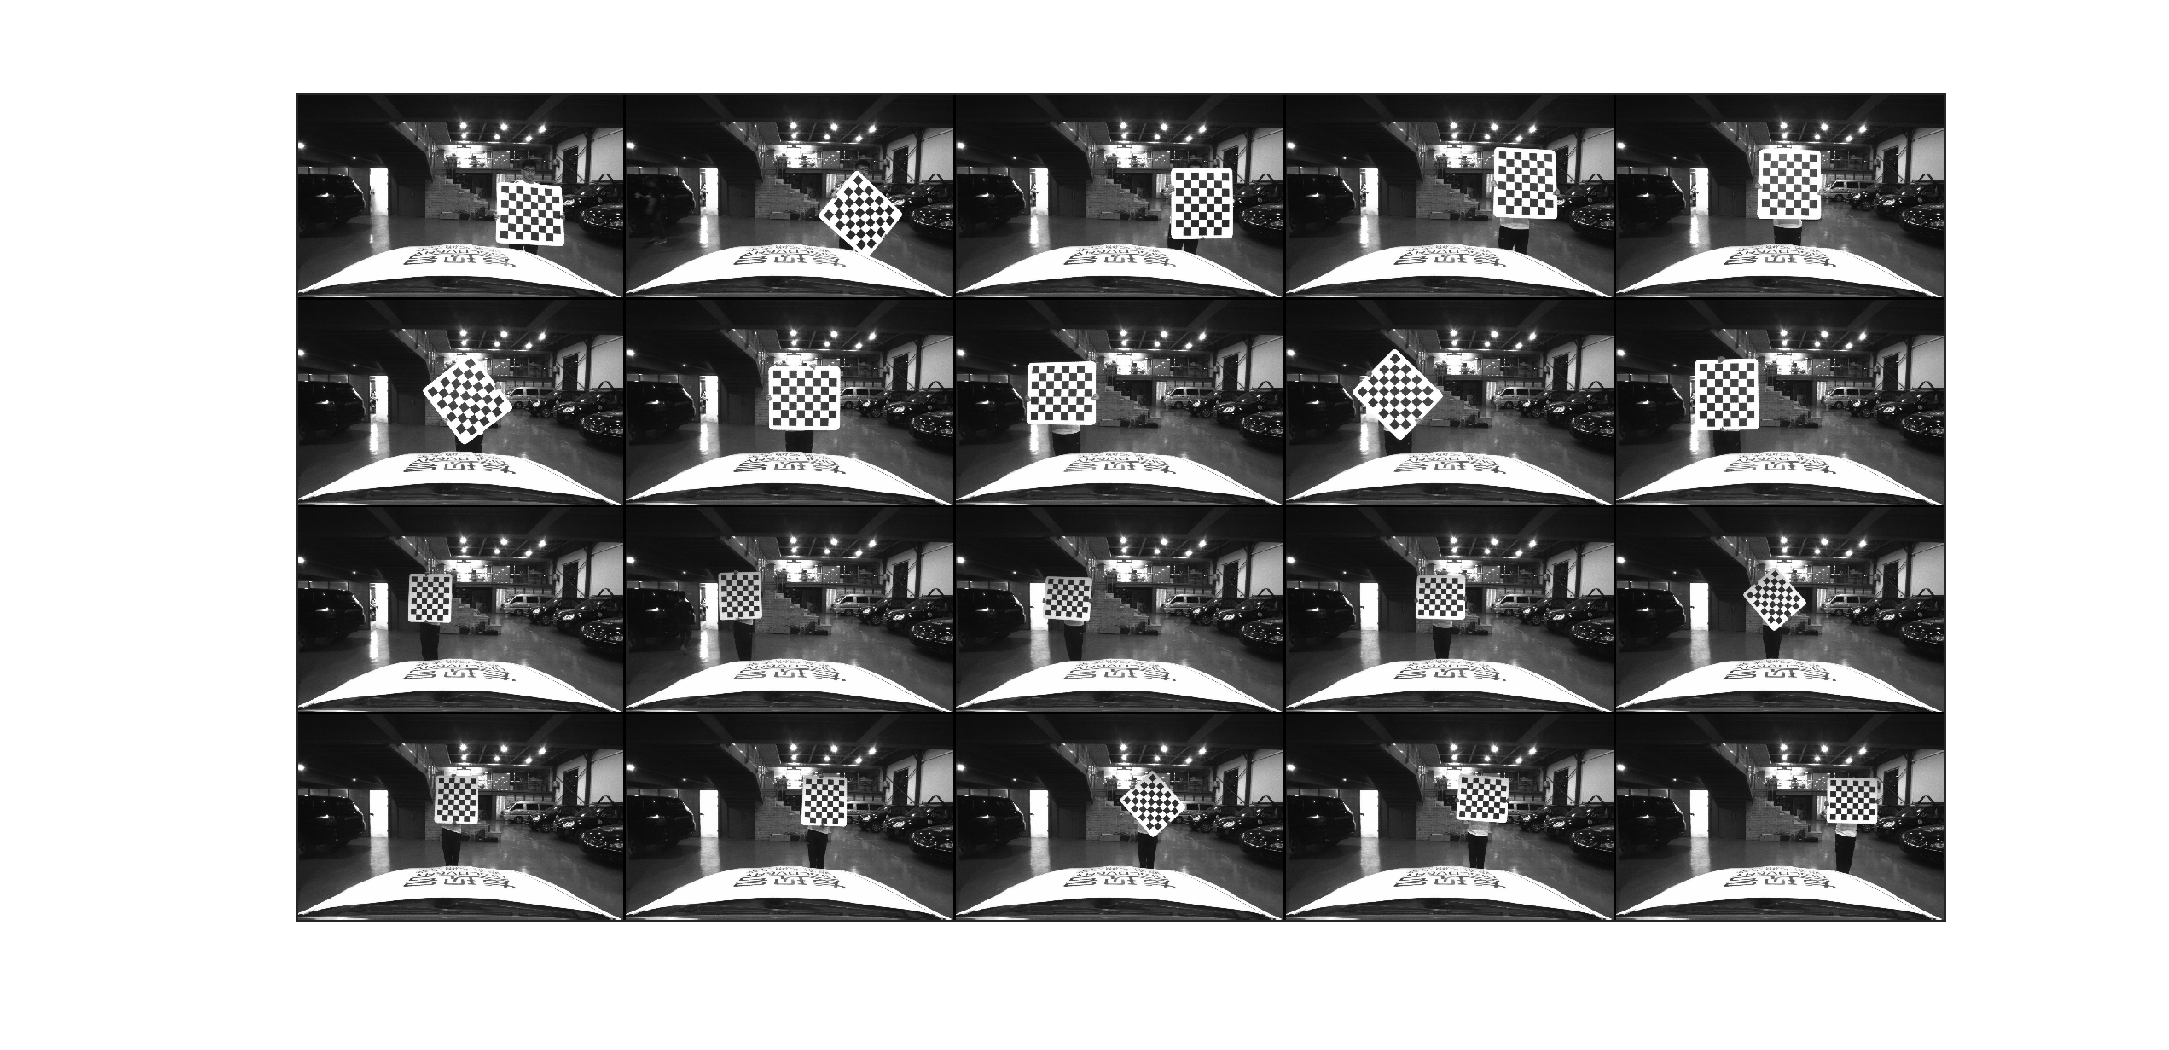
\includegraphics[width=16cm]{fig/data1.eps} \\
	\caption{标定板数据}\label{fig: calib}
\end{figure*}

\subsection{从LiDAR坐标系到相机坐标系}
已知标定板(世界坐标系)在相机坐标系下的位姿,要求解LiDAR坐标系和相机坐标系间的刚体变换关系,首先需得到LiDAR坐标系和
标定板间的刚体变换关系,因此,我们手动提取标定板的点云数据,并用最小二乘法进行拟合,得到该平面在LiDAR坐标系下位姿估计值
的“角-轴”值,即$\theta_{l,i}$和$\alpha_{l,i}$。然后,以LiDAR坐标系和相机坐标系下各标定平面到相机坐标系原点的
距离差的最小值为目标函数,优化该目标函数得到最优平移量,最后以LiDAR坐标系和相机坐标系下各标定平面到相机坐标系原点的
法向量夹角的最小值为目标函数,优化该目标函数得到最优旋转量。

相机坐标系原点平移t(LiDAR与相机间的距离)后,相机距标定平面的距离为$\alpha_{c,i}-\theta_{c,i}^{T}t$,
所以与平移量有关的目标函数如下:
\begin{equation}\label{eq1}
\begin{aligned}
& \min \limits_{t} \sum_{i=1}^{n}(\alpha_{l,i}-(\alpha_{c,i}-\theta_{c,i}^{T}t))^{2} \\
\Longrightarrow & t_{1}=\arg \min \limits_{t} || (\theta_{c}^{T}t-(\alpha_{l}-\alpha_{c}))||^{2}_{F} \\
\end{aligned}
\end{equation}
解 \eqref{eq1}, 即可得到平移量
$t_{1}=(\theta_{c}\theta_{c}^{T})^{-1}\theta_{c}(\alpha_{c}-\alpha_{l})$。

法向量夹角的最小值即夹角余弦的最大值,用正交旋转矩阵表示,则与旋转量有关的目标函数如下:
\begin{equation}\label{eq2}
\begin{aligned}
R_{1}=\arg \max \limits_{R} \sum_{i=1}^{n} \theta_{c,i}^{T} (R \theta_{l,i})
\end{aligned}
\end{equation}
其中,R是正交旋转矩阵,满足$R^{T}R=\vec{I}_{3}$,$det(R)=1$,对公式 \eqref{eq2}变形,将该问题转换成
典型的正交普鲁克问题(Orthogonal Procrustes Problem),如式下所示。
\begin{equation}\label{eq3}
\begin{aligned}
R_{1}=\max \limits_{R} trace(\theta_{c}^{T}R\theta_{l})
=\max \limits_{R} trace(R\theta_{l}\theta_{c}^{T})
\end{aligned}
\end{equation}
用奇异值分解(Singular Value Decomposition,SVD)的方法解\eqref{eq3},即可以得到旋转矩阵的解:
\begin{equation}
\begin{aligned}
R_{1}= VU^{T},  st.\theta_{l}\theta_{c}^{T}=USV^{T}
\end{aligned}
\end{equation}

以上的求解过程,我们仅使用点云数据估计了标定板平面参数值,为了更有效地利用点云数据并提高算法的鲁棒性,
我们使用点云平面拟合得到的内点进一步对上述过程中得到的LiDAR-Camera系统外参进行优化。

用$x_{l,i}$表示第i帧点云中拟合的标定板平面的内点,
即$x_{l,i}=[x_{l,i}^{(1)}, x_{l,i}^{(2)},...,x_{l,i}^{(m)}]$,$x_{l,i} \in R^{3x1}$,$m=m(i)$是
第i帧点云中拟合平面得到的内点的个数,则建立的统一旋转和平移量的目标函数如\eqref{eq4}所示,以上述$R_{1}$和$t_{1}$
为初值,优化该问题,得到粗标定过程的最终外参矩阵。
\begin{equation}\label{eq4}
\begin{aligned}
\arg \max \limits_{R,t} \sum_{i=1}^{n}\frac{1}{m(i)} 
\sum_{j=1}^{m(i)} (\theta_{c,i}^{T} (R x_{l,i}^{(j)}+t)-\alpha_{c,i})^{2}
\end{aligned}
\end{equation}

%%%%%%%%%%%%%%%%%%%%%%%%%%%%%%%%%%%%%%%%%%%%%%%%%%%%%%%%%%%%%%%%%%%%%%%%%%%%%%%%%%%%%%%%%
\section{LiADR-Camera联合细标定}
\label{sec:2}
将相机内参标定和LiDAR-Camera联合标定过程统一, 均使用棋盘格为靶标,方便采集实验数据,并降低了实验要求,简化了整个
标定流程。这种基于黑白棋盘格的离线标定方法虽然简单易实现,但是仍存在一些问题:
\begin{enumerate}[\indent (1)]
\item 标定精度难以保证;标定受光照和人为因素影响大,很多情况下的标定结果都不能满足后续点云和图像高精度融合的需要。
\item 标定误差无法更新和校正;这种基于特定靶标的离线标定方法,一旦标定结果发生偏移,都需要重新实验,过程繁琐,
无法满足无人驾驶系统在线感知算法的需求。
\end{enumerate}

综合考虑以上问题,我们用真实道路场景中的目标(人,树,路标,车等)作为LiDAR-Camera系统外标定的匹配模式,基于点云和图像
目标边缘对齐的融合结果,在线优化和更新该传感器系统外参。


\subsection{数据处理}
% 为保证所选点云和图像对边缘特征明显易于提取,需要人为选择数据采集场景或者人为对时间同步后的数据进行筛选。
3D点云和2D图像数据模态存在巨大差异,在进行边缘提取前,需先对点云减采样,取与相机视野重合扇区内的点云;并对点云进行
简单滤波,除去地面点(基于高度的滤波或者RANSAC)和非目标点(基于距离滤波或者检测算法)。然后,剪裁RGB图像,除去LiDAR
激光器扫描到的最高高度以外的图像区域,并根据图像剪裁的尺寸更新相机内参。最后处理得到如
\figurename\ref{fig: IDT-FIL}所示的图像和点云边缘。

\begin{figure*}[htbp]
	\centering
    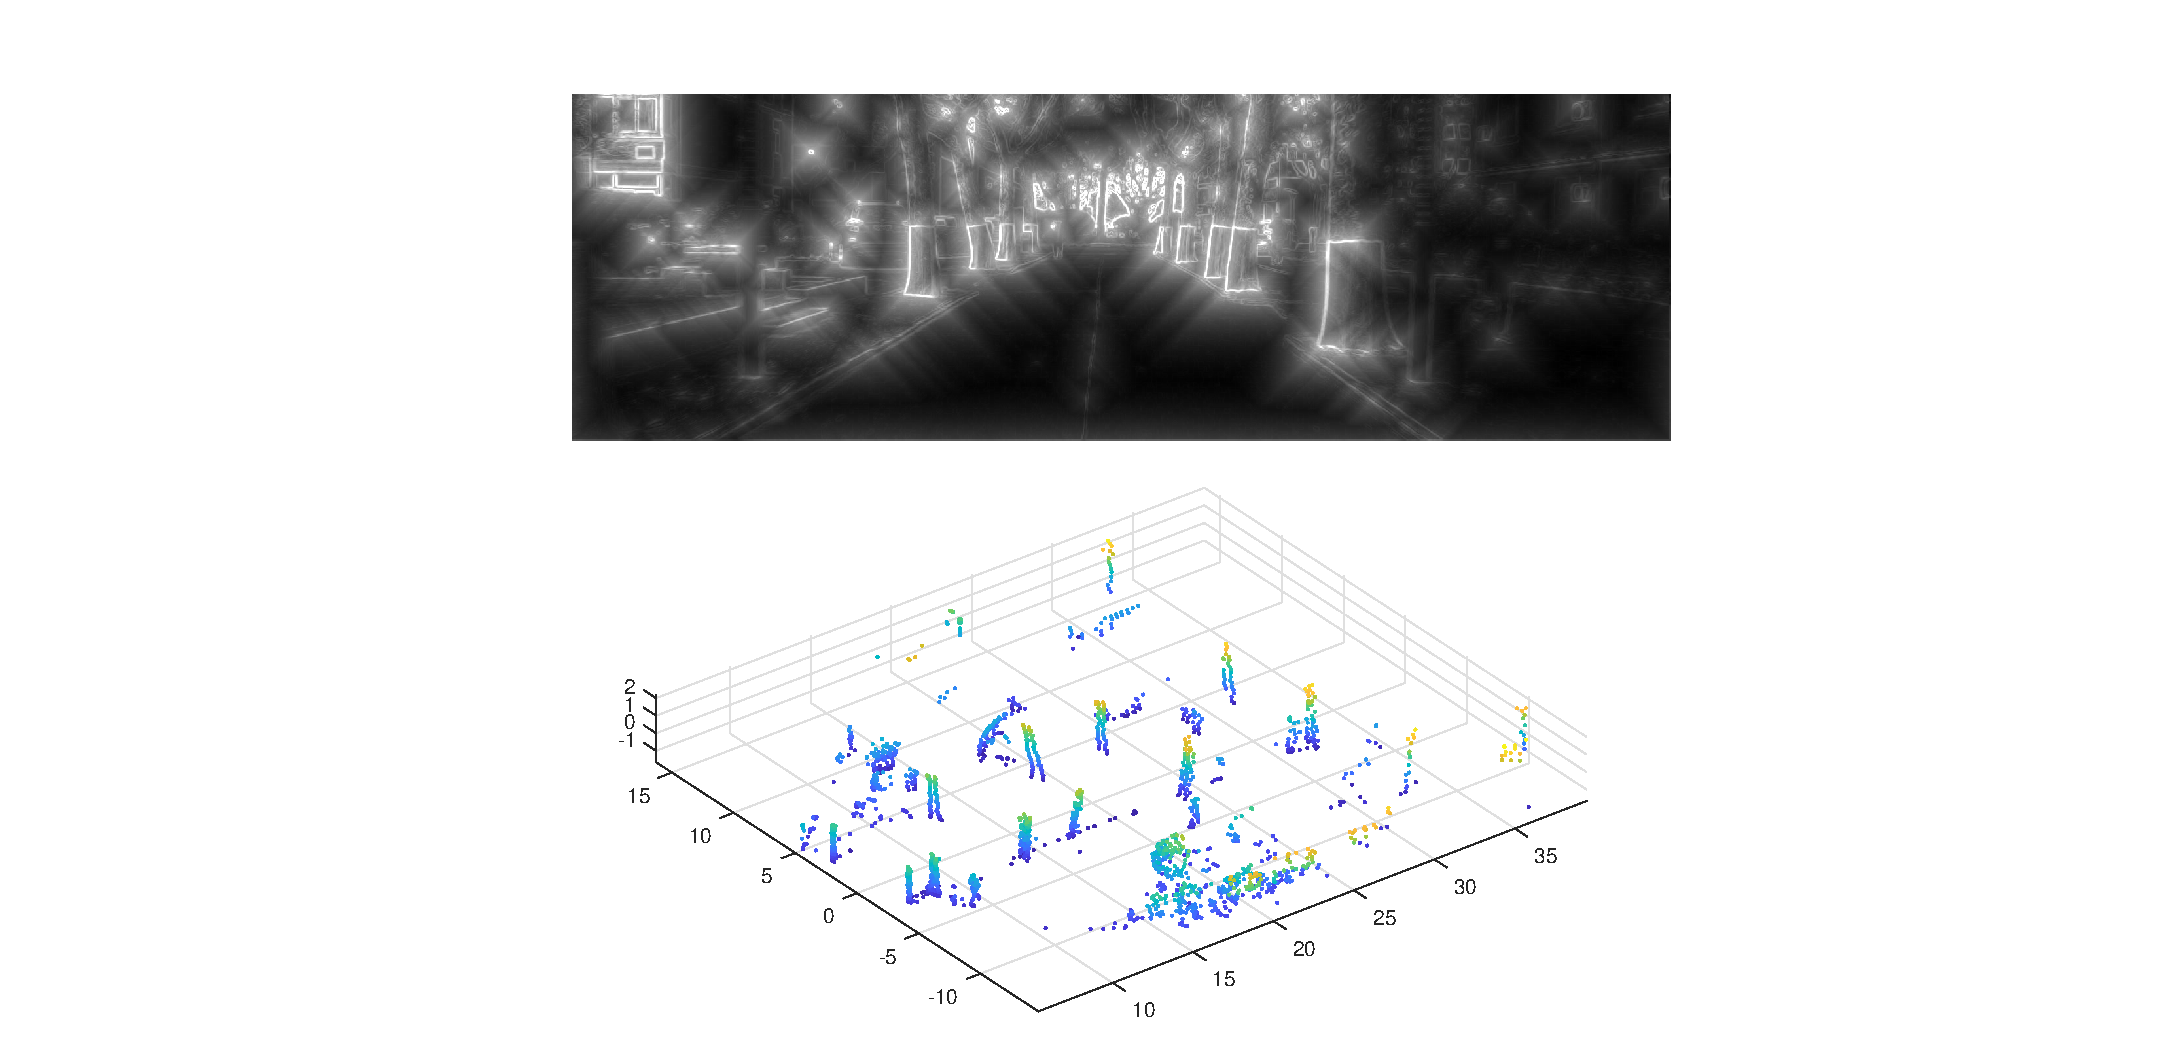
\includegraphics[width=18cm]{fig/IDT.eps} \\
	\caption{图像和点云边缘提取结果}\label{fig: IDT-FIL}
\end{figure*}

\subsubsection{点云边缘提取}
3D点云数据离散而稀疏,边缘不连续性明显,因此利用点云数据获取的边缘存在误差(与点云的分辨率有关)。
我们单独分析每帧点云中的每个激光器的返回数据,对于场景中的目标,由于视差和遮挡,则具有固定垂直扫射角的激光器的
返回数据中,与左右邻域点相比,越远的点越不可能是目标边缘点。基于该事实,建立式 \eqref{eq5}的点云边缘滤波指标。
\begin{equation}\label{eq5}
\begin{aligned}
X_i=\max(P_{i-1}^{r}-P_{i}^{r}, P_{i}^{r}-P_{i+1}^{r}, 0)^\gamma
\end{aligned}
\end{equation}
其中,$P_{i}^{r}$是返回的第i个点的深度值,$\gamma \in(0, 1)$是为提高近处点云权重而设置的参数,一般取经验值0.5。

对于Velodyne 64HDL LiDRA点云数据,我们以$X_i\ge 0.3m$为基准滤波提取点云数据中目标的边缘。


\subsubsection{图像边缘提取}
与点云边缘检测算法相比,图像边缘检测算法成熟,检测精度高,但仍然存在一些影响边缘匹配的问题,诸如由光照和阴影导致的
假边缘、离散孤立边,这些边难以滤波去除,因此除了人为选择标定场景(无强光和阴影的阴天或者傍晚等)外,我们对得到的边缘
图进行距离逆变换(inverse distance transform, IDT),提高真实边缘的比重并弥补点云边缘不连续性导致的边缘误差。
我们首先使用Sobel算子提取图像边缘,得到边缘图E,然后对E做IDT变换,变换过程如下:
\begin{equation}
\begin{aligned}
D_{i,j}=\alpha \cdot E_{i,j}+(1-\alpha)\cdot \max \limits_{x,y} E_{x,y}
\cdot \mu^{\max(|x-i|,|y-j|)} 
\end{aligned}
\end{equation}
其中,i, j, x, y为图像边缘E的像素索引,$\alpha$和$\mu$分别取经验值0.333和0.98。

\subsection{基于边缘匹配更新外参}
将粗标定过程中得到的旋转外参矩阵转换为欧拉角表示可以得到LiDAR-Camera系统的6DOF外参,
$C=(t_{x},t_{y},t_{z},\theta_{x},\theta_{y},\theta_{z})$,以此为初值,将点云投影到图像平面
可以建立与6DOF外参有关的目标函数,如下:
\begin{equation}\label{eq6}
\begin{aligned}
F_T=\sum_{f=1}^{n} \sum_{p=1}^{X^{f}} X_{p}^{f}\cdot D_{i,j}^{f}
\end{aligned}
\end{equation}
其中,n是选择用于实验的点云图像对的数量,$X^{f}$表示预处理后第f帧点云数据中点的个数,$(i,j)$表示第p个点投影到图像
平面的位置索引。

我们使用邻域搜索算法求解问题\eqref{eq6},得到更精确的外参。

%%%%%%%%%%%%%%%%%%%%%%%%%%%%%%%%%%%%%%%%%%%%%%%%%%%%%%%%%%%%%%%%%%%%%%%%%%%%%%%%%%%%%%
\section{标定流程}
\label{sec:3}

\subsection{数据采集与预处理}
\subsubsection{数据采集}

标定操作在MATLAB环境下进行,在Calibration文件夹下,包含CoarseCalibration、FineSearch、fToolBox、LCCT1、TOOLBOX$\_$calib五个文件夹。
CoarseCalibration文件夹下主要包含了img$\_$veloPreprocess.m和show.m两个文件,img$\_$veloPreprcoess根据筛选出的的图片来产生图片和点云对,show根据得到的标定矩阵来显示标定的结果。
FineSearch文件夹下主要包含了dataPreprocess.m和Search.m两个文件,dataPreprocess用来生成细标定搜索使用的数据,Search用来根据粗标定得到的结果和已有数据进一步优化标定矩阵,使之更为准确。
fToolBox文件夹主要包含了timeAlign.m,timeAlign用来对采集到的数据进行时间对齐并按时间顺序标号。
LCCT1文件夹为外参粗标定使用的工具箱文件夹。


TOOLBOX$\_$calib文件夹为相机内参标定使用的工具箱的文件夹。

% 在同样距离等条件下,激光对于白色材料反射强度最高,检测到的数据准确率最高。要求采集的标定板数据标定板平坦且边缘整齐。
% 我们采用的是7*8个边长为100mm的格子的标定板。

% 标定时保证相机与雷达前方区域平坦且光照条件柔和,无强光照射标定板。
% 将标定板朝向相机,以间距约0.5,1.5,2.5m围绕相机前方各个位置采集标定数据。

% 在VisualStudio下分别使用图像采集程序
% (img.cpp)与雷达数据采集程序(hdl.cpp)两个程序采集数据。

\subsubsection{时间同步}
采集数据后,使用MATLAB对数据进行预处理。首先进行时间同步:

\begin{enumerate}[$\star$]%项目符号开始
\item 使用文件: fToolBox$\verb|\|$timeAlign.m;
\item 部分代码片段如\figurename\ref{fig: timeAlign}所示;
\item 改其中的路径Path为存储标定数据的根文件夹;
\item 该程序会自动在根文件下创建dataSet文件夹,其中dataSet文件夹又包含img、velo、target、img$\_$select
四个子文件夹,分别用来存储时间对齐后的图像、时间对齐后的点云、筛选出用来标定的图片和点云对、筛选出的图片;
\item 点击“Run”运行,即可完成时间对齐,图像和点云分别以img$\_$xxxxxx.jpg和velo$\_$xxxxxx,
(xxxxxx为时间戳顺序的编号)存储在img和velo文件夹下。
\end{enumerate}

\begin{figure*}[htbp]
	\centering
    \includegraphics[width=12cm]{pic/TAL.png} \\
	\caption{时间同步代码片段}\label{fig: timeAlign}
\end{figure*}

\subsubsection{选取图片}
\begin{enumerate}[$\star$]%项目符号开始
\item 在img文件夹下,人工选择各个位置下的光照良好标定板无亮斑且边缘整齐的图片约40张放入img$\_$select文件夹内;
\item 使用MATLAB相机标定工具箱Camera Calibrator,图标与界面如\figurename\ref{fig: caca}所示。
\end{enumerate}

\begin{figure*}[htbp]
	\centering
    \includegraphics[width=8.5cm]{pic/2.png} \\
	\caption{Camera Calibrator图标与界面}\label{fig: caca}
\end{figure*}

具体操作流程如下:
% \begin{enumerate}[\indent $1)$]
% \item Add Images添加img$\_$select文件夹下的图片,点击“打开”;
% \item 弹出窗口如图3所示,Size of checkerbored square为标定板格子的边长,设定为100mm,点击“确定”;
% \item 点击Calibrate进行标定运算;
% \item 选择右侧Reprojection Errors中值较高的图片,即为我们可以筛掉的图片。
% 每次选择Reprojection Errors最高的一张图片,在img$\_$select文件夹中将其删除,并在界面中右键选择对应照片,
% 点击“Remove and Recalibrate”重新进行运算,如图4所示;
% \item 最后保留28-35张图片;
% \item 点击“Export Camera Parameters”保存工具箱计算得到的相机内参,为后续标定作参考;
% \end{enumerate}
\begin{enumerate}[\indent $1)$]
\item Add Images添加img$\_$select文件夹下的图片,点击“打开”;
\item 弹出窗口如\figurename\ref{fig: pic3}所示,Size of checkerbored square为标定板格子的边长,设定为100mm,点击“确定”;
\end{enumerate}

\begin{figure*}[htbp]
	\centering
    \includegraphics[width=8.5cm]{pic/3.png} \\
	\caption{设定标定板格子边长}\label{fig: pic3}
\end{figure*}

\begin{enumerate}[\indent $3)$]
\item 点击Calibrate进行标定运算;
\end{enumerate}

\begin{enumerate}[\indent $4)$]
\item 选择右侧Reprojection Errors中值较高的图片,即为我们可以筛掉的图片。
每次选择Reprojection Errors最高的一张图片,在img$\_$select文件夹中将其删除,并在界面中右键选择对应照片,
点击“Remove and Recalibrate”重新进行运算,如\figurename\ref{fig: pic4}所示;
\end{enumerate}

\begin{figure*}[htbp]
	\centering
    \includegraphics[width=12cm]{pic/4.png} \\
	\caption{删除图片并重新运算}\label{fig: pic4}
\end{figure*}

\begin{enumerate}[\indent $5)$]
\item 最后保留28-35张图片;
\end{enumerate}

\begin{enumerate}[\indent $5)$]
\item 点击“Export Camera Parameters”保存工具箱计算得到的相机内参,为后续标定作参考。
\end{enumerate}

图片筛选完成后,进行如下操作来生成最终标定使用的图片点云对:
\begin{enumerate}[$\star$]
\item 使用文件: CoarseCalibration$\verb|\|$img$\_$veloPreprocess.m,部分代码片段如\figurename\ref{fig: pic5}所示;
\item 修改其中的路径Path为标定数据文件夹下的dataSet文件夹;
\item 点击“Run”运行,即可找到选出的图片的对应激光点云,并保存在target文件夹里,
名称为laser$\_$targetX.xyz和img$\_$targetX.jpg。
\end{enumerate}

\begin{figure*}[htbp]
	\centering
    \includegraphics[width=8cm]{pic/5.png} \\
	\caption{img$\_$veloPreprocess部分代码片段}\label{fig: pic5}
\end{figure*}


\subsection{相机内参标定}
使用标定工具箱Matlab Calibration Toolbox:
\begin{enumerate}[$\star$]
\item 右键选择TOOLBOX$\_$calib文件夹,添加到路径$\rightarrow$选定的文件夹和子文件夹;
\item 将MATLAB当前文件夹设为target文件夹;
\item 命令行输入calib$\_$gui,出现界面如\figurename\ref{fig: pic6}所示,选择“Standard”;
\end{enumerate}

\begin{figure*}[htbp]
	\centering
    \includegraphics[width=8cm]{pic/6.png} \\
	\caption{初始界面}\label{fig: pic6}
\end{figure*}

\begin{enumerate}[$\star$]
\item 出现界面如\figurename\ref{fig: pic7}所示,选择“Image Names”;
\end{enumerate}

\begin{figure*}[htbp]
    \centering
    \includegraphics[width=10cm]{pic/7.png} \\
    \caption{工具箱界面}\label{fig: pic7}
\end{figure*}

\begin{enumerate}[$\star$]
\item 命令行出现“Basename camera calibration images (without number nor suffix):”,
此时需要输入图像基础名称,所以在命令行输入“img$\_$target”,回车;
\item 命令行出现“Image format: ([]='r'='ras', 'b'='bmp', 't'='tif', 'p'='pgm', 'j'='jpg', 'm'='ppm')”,
此时需要选择图像格式,所以输入“j”,回车;
\item 图片加载完成后,选择“Extract Grid Corners”,命令行出现“Number(s) of image(s) to process
 ([] = all images) =”,回车默认选择全部图片;
\item 命令行出现“wintx ([] = 15) =”和“winty ([] = 15) =”,即为选择窗口大小,两次回车即可;
\item 命令行出现“Do you want to use the automatic square counting mechanism 
(0=[]=default)or do you always want to enter the number of squares manually (1,other)?”,回车即可;
\item 弹出窗口中,接下来需要选择标定板的四个角点,选定其中一角作为原点,每次按照该原点按顺时针围一个框,
如\figurename\ref{fig: pic8}(1)所示,选好后回车确认,命令行出现“Size dX of each square along the X direction 
([]=100mm) =  Size dY of each square along the Y direction ([]=100mm) =”,回车确认,
此时出现角点检测后的结果,如\figurename\ref{fig: pic8}(2)所示
\end{enumerate}

\begin{figure*}[htbp]
    \centering
    \includegraphics[width=14cm]{pic/8.pdf} \\
    \caption{(1)选择标定板角点 (2)角点检测结果}\label{fig: pic8}
\end{figure*}

\begin{enumerate}[$\star$]
\item 命令行出现“Need of an initial guess for distortion? ([]=no, other=yes)”,
再次回车出现下一张图,重复上述操作直到所有图片检测完毕;
\item 选择“Calibration”进行相机内参标定运算;
\item 选择“Save”,保存结果,会在target文件夹下生成名称为Calib$\_$Result.mat的文件。
\end{enumerate}

\subsection{LiDRA-Camera联合粗标定}
使用LCCT工具箱标定LiDRA-Camera系统初始外参:

\begin{enumerate}[$\star$]
\item 右键选择LCCT1下的src文件夹,添加到路径$\rightarrow$选定的文件夹和子文件夹;
\item 将MATLAB当前文件夹设为target文件夹;
\item 命令行输入lasercamcalib,出现界面如\figurename\ref{fig: pic9}所示;
\item 选择“Select a camera calib file”,选择Calib$\_$Result.mat;
\item 选择“Search scan files”,命令行出现“Enter base name of scans (without numbers or suffix):”,
即选择点云文件基础名称,输入laser$\_$target,回车;
\item 命令行出现“Enter suffix of scan files ([] = "xyz"):”,即选择点云文件扩展名,直接回车即可;
\item 选择“List active”;
\item 选择“Select planes”,命令行出现“Enter indices of range images to preview ([]=all active):”,
直接回车即可;
\item 命令行出现“use range image (r) or 3D point cloud (p) to select checkboard plane?
 (default:p):”,此时需要选择选定标定板的方法,我们选择rang image的方式,故输入r,回车;
\end{enumerate}

\begin{figure*}[htbp]
    \centering
    \includegraphics[width=6cm]{pic/9.png} \\
    \caption{LCCT工具箱界面}\label{fig: pic9}
\end{figure*}

\begin{enumerate}[$\star$]
\item 出现图片窗口如\figurename\ref{fig: pic10}所示,选择Select plane,左键选择标定板角点,
ESC可以取消之前的选定,选好后右键确认;
\end{enumerate}

\begin{figure*}[htbp]
    \centering
    \includegraphics[width=9cm]{pic/10.png} \\
    \caption{选择标定板平面区域}\label{fig: pic10}
\end{figure*}

\begin{enumerate}[$\star$]
\item 选择“Next”,然后重复操作,直至处理完所有图片;
\item 选择“Save$\&$Quit”;
\item 在工具箱界面选择“Calibrate”进行标定运算;
\item 选择“Save”,输入要保存的名字,回车即可保存。
\end{enumerate}

\subsection{LiDRA-Camera联合细标定}
执行搜索算法前,先处理用于搜索的数据:
\begin{enumerate}[$\star$]
\item 预选选取5-15对时间同步后边缘明显的点云-图像数据,保存在FineSearch$\verb|\|$Data$\verb|\|$ORGData目录中;
\item 运行FineSearch目录下数据处理文件dataPreprocess.m,调用IDT.m函数处理图像,
调用PC$\_$filter.m函数处理点云,将得到的图像边缘和点云边缘保存于结构体数据Data.mat中,
存于FineSearch$\verb|\|$Data目录下;
\item 调用自定义工具箱fToolBox中Rt2C.m将粗标定过程中得到的外参矩阵用6DOF外参C表示;
\end{enumerate}

得到图像和点云边云后,使用搜索算法精确标定传感器系统外参:

\begin{enumerate}[$\star$]
\item 初始化FineSearch目录下Search.m函数中的内参K$\_$int和外参C;
\item 更新搜索步长delta$\_$t和delta$\_$R;
\item 执行Search.m文件;
\item 搜索的关键代码片段如\figurename\ref{fig: pic11}所示。
\end{enumerate}

\begin{figure*}[htbp]
    \centering
    \includegraphics[width=13cm]{pic/11.png} \\
    \caption{Search.m代码片段}\label{fig: pic11}
\end{figure*}

%%%%%%%%%%%%%%%%%%%%%%%%%%%%%%%%%%%%%%%%%%%%%%%%%%%%%%%%%%%%%%%%%%%%%%%%%%%%%%%%%%%%%%%%%%%
\section{标定注意事项}

\begin{enumerate}[\indent $1)$]
\item 制作棋盘格靶标时应特别注意,黑色方格与白色方格尺寸需要相同,而且所有方格的尺寸必须严格一致。
靶标的方格数量不宜太小,行数和列数以大于7为宜。方格的尺寸不宜太大或太小,采集的整幅靶标图像中方格的边长尺寸不小于
20像素。
\item 采集靶标图像时应特别注意,需要在不同的角度不同的位置采集靶标的多幅图像。
采集到的图像必须清晰,靶标图像尺寸以占整幅图像尺寸的1/3-3/4为宜。靶标
图像最好在整幅图像的不同位置都有分布,不宜过于集中于同一区域。靶标放置位
置与摄像机之间的距离最好为视觉系统的主要工作距离。靶标相对于摄像机的角度
应有较大范围的变化,应包含绕三个轴较大角度的旋转,最好不小于30度。采集
的靶标图像数量不应太少,建议以20-35幅靶标图像为宜。
\item 内参标定,提取角点时,在图形窗口利用鼠标点击设定棋盘格靶标的选定区域。点击的第一个
角点作为靶标坐标系的原点,顺序点击 4 个角点形成四边形。相邻两次点击的角点应在同一条网格线上,
使得所形成的四边形的边应与棋盘格靶标的网格线基本平行。为提高点击的角点的精度,
建议将显示靶标图像的图像窗口放大到最大,利用
鼠标的十字标线尽可能准确的点击4个角点。
\item 外参标定,提取角点时,在图形窗口利用鼠标点击的第一个角点作为靶标坐标系的原点,得到
的外参数是靶标坐标系在摄像机坐标系中的位姿。
\item 采集细标定数据时,避免强光和阴影,建议傍晚和阴天采集数据。
\end{enumerate}

%\appendix
%\include{appendix}

% \backmatter%%%%%%%%%%%%%%%%%%%%%%%%%%%%%%%%%%%%%%%%%%%%%%%%%%%%%%%
% \include{solutions}
% \include{referenc}
% \printindex

%%%%%%%%%%%%%%%%%%%%%%%%%%%%%%%%%%%%%%%%%%%%%%%%%%%%%%%%%%%%%%%%%%%%%%

\end{document}





